\documentclass[11pt,a4paper,fontset=none]{ctexart}
\usepackage[margin=1in]{geometry}
\usepackage{fontspec}
\setCJKmainfont{Noto Serif CJK SC}[BoldFont={Noto Serif CJK SC Bold}]
\setCJKsansfont{Noto Sans CJK SC}
\setCJKmonofont{Noto Sans Mono CJK SC}
\usepackage{amsmath,amssymb,amsfonts}
\usepackage{graphicx,booktabs,float,caption,xcolor,listings}
\usepackage[hidelinks]{hyperref}
\usepackage{microtype}
\captionsetup{font=small}
\setcounter{tocdepth}{1}
\lstset{language=Python,basicstyle=\ttfamily\scriptsize,keywordstyle=\color{blue!70!black},
commentstyle=\color{green!40!black},stringstyle=\color{red!60!black},
numbers=left,numberstyle=\tiny\color{gray},numbersep=6pt,showstringspaces=false,
breaklines=true,frame=single,rulecolor=\color{black!40},tabsize=4}
\newcommand{\GBMEMRate}{0.500}
\newcommand{\GBMEMWeakRate}{0.999}
\newcommand{\GBMMilRate}{0.991}
\newcommand{\GBMMilWeakRate}{1.000}
\newcommand{\GBMAnalyticWeakRate}{0.9993}
\newcommand{\GBMFitWindow}{$N=64,128,256,512,1024$}
\newcommand{\GBMExactMean}{105.1987}
\newcommand{\GBMExactVariance}{1045.0120}
\newcommand{\GBMExactMeanCI}{[105.0403, 105.3571]}
\newcommand{\NARate}{0.491}
\newcommand{\NAFitWindow}{$N=8,16,32,64$}
\newcommand{\NAExactMean}{105.08796}
\newcommand{\NAExactMeanCI}{[104.89962, 105.27629]}
\newcommand{\NAPayoff}{14.53804}
\newcommand{\NAPayoffCI}{[14.40515, 14.67093]}
\newcommand{\NAWeakInterpretation}{在 $N=8,16,32$ 时，区间不含零，因此这些较粗网格的收益差可以从抽样噪声中分辨。在 $N=64,128,256$ 时，区间包含零，现有样本无法可靠判断偏差符号。这不证明偏差为零，也不足以为完整网格范围指定弱阶。}
\newcommand{\NAReferenceInterpretation}{相邻参考网格的平均绝对差从 2048 与 4096 步时的 0.05679，降至 4096 与 8192 步时的 0.04016，后者约为前者的 0.707 倍，与半阶缩放相容。在 $N=8,16,32,64$ 的拟合窗口内，0.04016 约占粗网格到最细参考强差的 3.2\% 至 8.9\%；在 $N=128,256$ 时，这一比例升至 12.6\% 和 18.0\%。因此，更细的粗网格相对更受参考分辨率影响，主要斜率使用参考影响相对较小的四个网格。这些比较衡量参考加密的敏感性，不构成相对于未知精确解的误差上界。}

\title{金融随机微分方程的数值模拟\\
\large 第四题：GBM 基准与非仿射波动率}
\author{课程作业报告（中文译本）}
\date{2026 年 9 月}
\begin{document}
\maketitle
\begin{abstract}
本文比较几何布朗运动（GBM）的精确模拟、Euler--Maruyama（EM）方法和 Milstein 方法，并研究一个需要数值参考解的非仿射随机波动率模型。所有离散方法都通过聚合布朗增量使用共同随机路径。对于 GBM，终值强收敛的测量阶数为 \GBMEMRate{}（EM）和 \GBMMilRate{}（Milstein），与理论上的 $1/2$ 阶和 $1$ 阶一致。我们使用配对差、独立拟合的控制变量和解析的离散均值公式，将弱均值偏差与蒙特卡洛抽样不确定性分开；终值分布则与精确的对数正态分布比较。对于非仿射模型，我们对数价格和波动率因子都使用 EM，因此模拟价格保持为正。给定拟合窗口上的经验强阶为 \NARate{}。我们用置信区间和三层嵌套参考网格报告收益偏差；当偏差无法由抽样误差中分辨出来时，不强行指定弱收敛阶。实验说明：精确基准可以验证方法，而数值网格之间的一致只能通过参考网格加密来评估。
\end{abstract}
\tableofcontents
\vfill
\noindent\small 可复现性：随报告提供完整 Python 源码、随机种子、数值表格、图形和运行记录。报告中的置信区间是逐点蒙特卡洛区间。

\newpage
\section{引言与理论背景}
题目给出的 SDE 方向要求研究强收敛、弱收敛、抽样不确定性以及嵌套网格验证；这些内容取代了确定性 ODE 中的稳定域和自适应步长分析~\cite{pack}。GBM 有精确的路径基准，而题目规定的非仿射模型必须把时间离散作为模型求解的一部分。本文的目标是说明实验真正验证了什么，而不是根据看起来合理的样本路径猜测精度。

\subsection{GBM 及其精确转移}
当 $S_0>0$ 时，It\^o 随机微分方程和对数变换为
\begin{align}
dS_t&=\mu S_t\,dt+\sigma S_t\,dW_t,\\
dX_t&=(\mu-\tfrac12\sigma^2)\,dt+\sigma\,dW_t,\qquad X_t=\log S_t.
\end{align}
It\^o 修正项非常重要：漏掉 $-\sigma^2/2$ 会改变价格均值。积分得到
\begin{equation}
S_t=S_0\exp\{(\mu-\tfrac12\sigma^2)t+\sigma W_t\}.
\label{eq:exact}
\end{equation}
因此 $S_T$ 服从对数正态分布，且
\begin{align}
m&=\mathbb E[S_T]=S_0e^{\mu T},\\
v&=\operatorname{Var}(S_T)=S_0^2e^{2\mu T}(e^{\sigma^2T}-1),\\
q_p&=S_0\exp\{(\mu-\tfrac12\sigma^2)T+\sigma\sqrt{T}\Phi^{-1}(p)\}.
\end{align}
对于本文选择的 GBM 基准 $S_0=100$、$\mu=0.05$、$\sigma=0.30$、$T=1$，理论均值为 $105.1271$，方差为 $1040.7868$（四舍五入）。GBM 参数是实验选择；非仿射模型的参数由题目规定。

\subsection{在同一条布朗路径上比较三种方法}
令 $h=T/N$，$\Delta W_n\sim N(0,h)$。精确模拟使用
\begin{equation}
S_{n+1}=S_n\exp\{(\mu-\tfrac12\sigma^2)h+\sigma\Delta W_n\}.
\end{equation}
基于价格的 EM 和标量 Milstein 更新分别为
\begin{align}
S_{n+1}^{E}&=S_n^{E}(1+\mu h+\sigma\Delta W_n),\label{eq:em}\\
S_{n+1}^{M}&=S_n^{M}\{1+\mu h+\sigma\Delta W_n+
\tfrac12\sigma^2[(\Delta W_n)^2-h]\}.\label{eq:mil}
\end{align}
额外项来自 $\tfrac12 b(S)b'(S)[(\Delta W)^2-h]$，其中 $b(S)=\sigma S$~\cite{higham}。在通常的正则性假设下，终值强阶分别为 $1/2$ 和 $1$；对于合适的光滑测试函数，弱阶为 $1$。如果把 EM 直接用在 GBM 的对数价格上，网格点处的转移反而是精确的，因为噪声是加性的，Milstein 修正为零，无法用它验证非平凡的一阶比较。

\newpage
\section{蒙特卡洛方法}
\subsection{耦合与不确定性}
先在最细网格上生成独立路径。粗网格的一个布朗增量等于对应细增量之和：
\begin{equation}
\Delta W_n^{(h)}=\sum_{j=nr}^{(n+1)r-1}\Delta W_j^{(\delta)},
\qquad h=r\delta.
\label{eq:coupling}
\end{equation}
对于 GBM，精确终值使用同一个总增量 $W_T$。对于非仿射模型，粗网格和参考网格也使用配对的布朗驱动。如果每个分辨率都独立生成随机数，路径之间会保留一个不随步长消失的差异，强收敛实验就失去了意义。

对 $M$ 条独立路径，定义 $A_i(h)=|S_{T,i}^{(h)}-S_{T,i}^{\rm ref}|$。终值 $L^1$ 强误差估计量及其近似 95\% 区间为
\begin{equation}
\widehat e_s(h)=M^{-1}\sum_i A_i(h),\qquad
\widehat e_s(h)\ \pm\ 1.96\,s_A/\sqrt M.
\end{equation}
经验阶数是在明确给定的拟合窗口上，对 $\log\widehat e_s$ 关于 $\log h$ 做最小二乘拟合所得斜率。由于不同步长之间共享随机路径，点之间相关；这里的斜率是描述性结果，并没有声称有独立回归的置信区间。

对于收益函数 $\varphi$，使用带符号的配对差
\begin{equation}
D_i(h)=\varphi(S_{T,i}^{(h)})-\varphi(S_{T,i}^{\rm ref}),\qquad
\widehat b(h)=\overline D,\qquad
{\rm CI}_{95}=\overline D\pm1.96\,s_D/\sqrt M.
\end{equation}
弱误差是 $|\mathbb E[D]|$，不是 $\mathbb E|D|$。即使区间跨过零，也保留这个带符号的结果。这些区间只量化抽样误差，不包括数值参考本身的时间离散偏差。

\subsection{解析 GBM 的弱均值偏差}
对于两种方法，条件期望下的乘子都是 $1+\mu h$。因此
\begin{align}
\mathbb E[S_N^{E}]=\mathbb E[S_N^{M}]&=S_0(1+\mu h)^{T/h},\\
b_{\rm exact}(h)&=S_0(1+\mu h)^{T/h}-S_0e^{\mu T},\label{eq:weak}\\
b_{\rm exact}(h)&=-\tfrac12 S_0e^{\mu T}\mu^2T\,h+O(h^2).
\end{align}
这说明当前非退化参数下，均值偏差为一阶。这是验证目标，不是把解析答案替换成蒙特卡洛估计。

模拟还构造了均值为零的控制变量 $C_i$，并估计 $\overline{D-\beta^\top C}$。系数 $\beta$ 在独立的预实验样本上拟合，然后固定用于正式样本，因此正式估计仍保持无偏；预实验不计入报告的正式路径数。完整控制变量公式和实现保留在随附的 \texttt{gbm.py} 中。

\newpage
\section{模型与实验方案}\label{sec:protocol}
\subsection{非仿射随机波动率}
令 $X=\log S$，题目规定的系统为
\begin{align}
dX_t&=\{\mu-\tfrac12g(Y_t)^2\}\,dt+g(Y_t)\,dW_t^{(1)},\\
dY_t&=\kappa(\theta-Y_t)\,dt+\xi\sqrt{1+Y_t^2}\,dW_t^{(2)},\\
g(y)&=\sigma_{\min}+\frac{\sigma_{\max}-\sigma_{\min}}{1+e^{-y}},
\qquad d\langle W^{(1)},W^{(2)}\rangle_t=\rho\,dt.
\end{align}
\begin{table}[H]\centering
\caption{题目规定的非仿射基准参数。}
\begin{tabular}{cccccc}\toprule
$S_0$ & $Y_0$ & $\mu$ & $\kappa$ & $\theta$ & $\xi$\\\midrule
100 & 0 & 0.05 & 2 & $-0.2$ & 0.6\\\midrule
$\rho$ & $\sigma_{\min}$ & $\sigma_{\max}$ & $T$ & $X_0$ & 行权价 $K$\\\midrule
$-0.7$ & 0.10 & 0.50 & 1 & $\log 100$ & 100\\\bottomrule
\end{tabular}
\end{table}
从相互独立的标准正态变量 $Z_1,Z_2$ 出发，生成
\begin{equation}
\Delta W^{(1)}=\sqrt h Z_1,\qquad
\Delta W^{(2)}=\sqrt h(\rho Z_1+\sqrt{1-\rho^2}Z_2).
\end{equation}
实现的 EM 步是在左端点同时更新：
\begin{align}
X_{n+1}&=X_n+[\mu-\tfrac12g(Y_n)^2]h+g(Y_n)\Delta W_n^{(1)},\\
Y_{n+1}&=Y_n+\kappa(\theta-Y_n)h+\xi\sqrt{1+Y_n^2}\Delta W_n^{(2)},\\
S_{n+1}&=\exp(X_{n+1}).
\end{align}
两条更新式都使用旧值 $Y_n$。如果先更新 $Y$，再用 $Y_{n+1}$ 更新第一条式子，就改变了离散方法。稳定实现的 logistic 函数避免指数溢出；程序还检查状态有限以及价格为正。

\subsection{网格与可复现性}
\begin{table}[H]\centering\small
\caption{计算方案；所有网格都是 2 的幂次嵌套网格。}\label{tab:protocol-cn}
\begin{tabular}{lrlr}\toprule
项目 & 数值 & 项目 & 数值\\\midrule
GBM 正式路径数 & 160,000 & 独立预实验路径数 & 20,000\\
GBM 随机种子 & 2026090804 & 预实验种子 & 2026090805\\
GBM 网格 $N$ & 8 至 1024 & GBM 批大小 & 2000\\
非仿射路径数 & 100,000 & 随机种子 & 2026090804\\
粗网格 $N$ & 8,16,32,64,128,256 & 参考网格 $N$ & 2048,4096,8192\\
GBM 耗时 & 30.9 秒 & 非仿射耗时 & 107.8 秒\\
\bottomrule\end{tabular}
\end{table}

所有计算使用双精度和固定的 NumPy 随机数生成器；正式路径分批处理，以限制内存。随机种子、批大小、软件版本、耗时和完整精度结果都保存在 JSON 文件中。实验不使用外部市场数据。GBM 在价格变量上比较精确解、EM 与 Milstein；非仿射模型使用逐渐加密的 EM 参考。收益函数为 $\varphi(S)=(S-100)^+$，即在题目给定漂移下的\emph{未贴现期望看涨收益}。没有定价测度和贴现率，因此不将它解释为风险中性期权价格。

\newpage
\section{GBM 数值结果}
\subsection{强收敛}
\begin{figure}[H]\centering
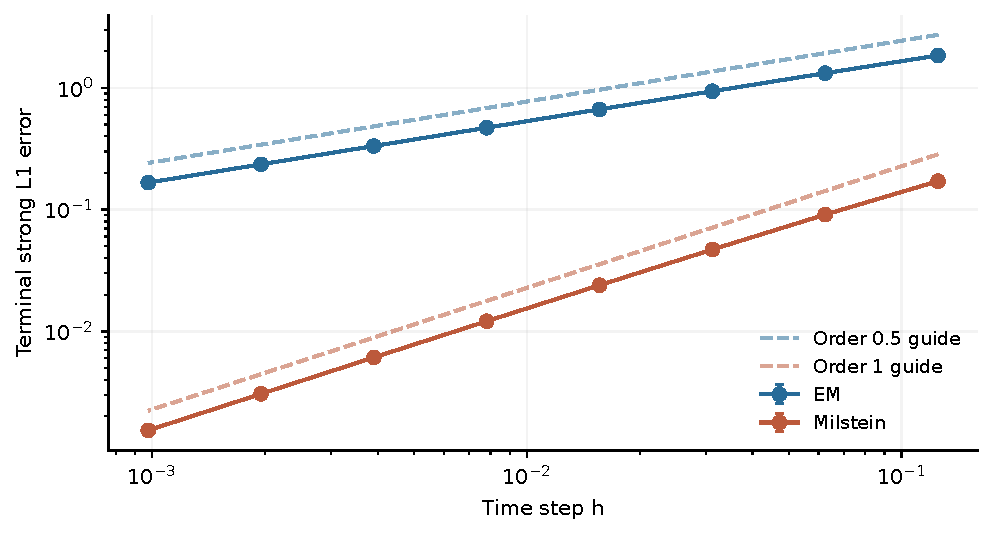
\includegraphics[width=.92\textwidth]{figures/report_gbm_strong.pdf}
\caption{耦合 GBM 的终值 $L^1$ 误差。误差棒是逐点 95\% 蒙特卡洛区间，许多区间小于标记。参考线表示 $1/2$ 阶和 $1$ 阶。}
\end{figure}
\begin{table}[H]\centering\small
\caption{GBM 强误差估计及 95\% 区间半宽。}\label{tab:gbm-strong-cn}
\begin{tabular}{rrr}\toprule
$h$ & EM & Milstein\\\midrule
1/8 & $1.84750\pm0.00809$ & $0.17127\pm0.00100$\\
1/16 & $1.32218\pm0.00562$ & $0.09096\pm0.00048$\\
1/32 & $0.93847\pm0.00396$ & $0.04697\pm0.00023$\\
1/64 & $0.66641\pm0.00278$ & $0.02391\pm0.00011$\\
1/128 & $0.47071\pm0.00196$ & $0.01209\pm0.00006$\\
1/256 & $0.33297\pm0.00139$ & $0.00610\pm0.00003$\\
1/512 & $0.23550\pm0.00098$ & $0.00306\pm0.00001$\\
1/1024 & $0.16658\pm0.00069$ & $0.00153\pm0.00001$\\
\bottomrule\end{tabular}
\end{table}

在窗口 $\GBMFitWindow{}$ 上，EM 和 Milstein 的拟合斜率分别为 \GBMEMRate{} 和 \GBMMilRate{}。这与理论区别一致：EM 没有包含二次随机增量，而 Milstein 加入了该项。在最细步长下，Milstein 的路径误差明显更小。由于两种方法使用完全相同的布朗路径，差异来自更新公式，而非不同随机实现。

精确解在模拟网格点上没有时间离散误差。重新排列求和可能造成极小的浮点差异，但那不是收敛阶。这里比较的是终值误差，而不是整条路径上的最大误差；后者是另一种诊断。

\newpage
\subsection{弱收敛与方差缩减}\label{sec:gbmweak}
\begin{figure}[H]\centering
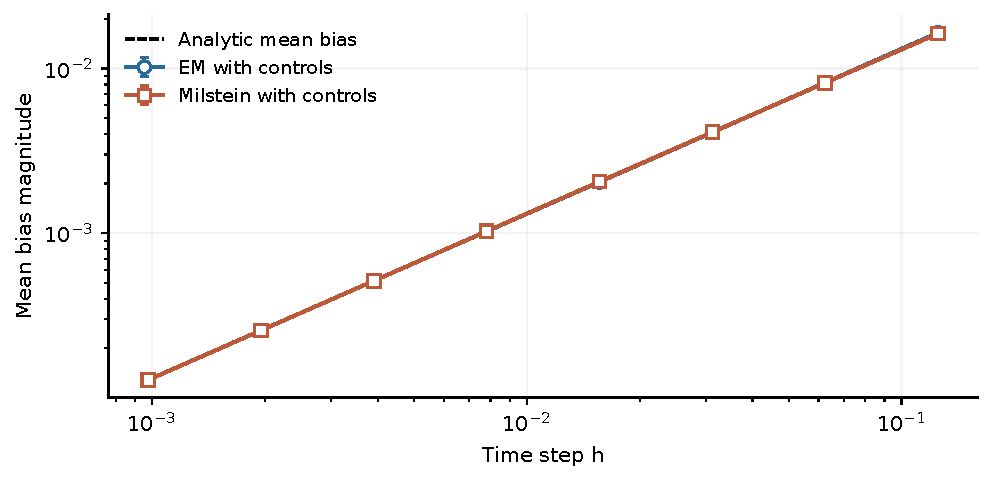
\includegraphics[width=.92\textwidth]{figures/report_gbm_weak.pdf}
\caption{GBM 均值偏差的大小。图中将控制变量后的配对估计与解析离散均值偏差比较；原始估计和区间保留在数值表中。}
\end{figure}
\begin{table}[H]\centering\small
\caption{带符号的弱偏差；表中给出控制后的估计和 95\% 区间半宽。}\label{tab:gbm-weak-cn}
\begin{tabular}{rrrr}\toprule
$h$ & 解析偏差 & EM（控制后） & Milstein（控制后）\\\midrule
1/8 & $-1.636\times10^{-2}$ & $-1.649\times10^{-2}\pm1.940\times10^{-4}$ & $-1.629\times10^{-2}\pm9.901\times10^{-5}$\\
1/32 & $-4.102\times10^{-3}$ & $-4.096\times10^{-3}\pm2.811\times10^{-5}$ & $-4.106\times10^{-3}\pm1.399\times10^{-5}$\\
1/128 & $-1.026\times10^{-3}$ & $-1.025\times10^{-3}\pm3.653\times10^{-6}$ & $-1.027\times10^{-3}\pm1.810\times10^{-6}$\\
1/512 & $-2.566\times10^{-4}$ & $-2.567\times10^{-4}\pm4.660\times10^{-7}$ & $-2.566\times10^{-4}\pm2.301\times10^{-7}$\\
1/1024 & $-1.283\times10^{-4}$ & $-1.284\times10^{-4}\pm1.649\times10^{-7}$ & $-1.283\times10^{-4}\pm8.144\times10^{-8}$\\
\bottomrule\end{tabular}
\end{table}

虽然两种方法的强误差不同，但它们的解析均值偏差相同。解析偏差的拟合阶数为 \GBMAnalyticWeakRate{}；在给定数据上，控制后的蒙特卡洛斜率为 \GBMEMWeakRate{} 和 \GBMMilWeakRate{}。这些结果要结合区间解读，不能代替式~\eqref{eq:weak}。在很小的 $h$ 下，未经控制的 EM 配对估计噪声太大，难以可靠分辨这个小偏差。

控制变量的作用是减少抽样噪声而不改变估计目标。如果 $C$ 的均值已知为零，那么对固定 $\beta$ 有 $\mathbb E[D-\beta C]=\mathbb E[D]$；选择与 $D$ 相关的 $C$ 可以显著降低样本平均的方差。实现使用五个由同一批布朗增量计算的控制变量，在独立的 20,000 条预实验路径上拟合系数，再固定到 160,000 条正式路径上。它们是降噪工具，不是新的收敛方法。

在 $N=1024$ 的 EM 实验中，原始配对标准误约为 $5.46\times10^{-4}$，大于解析偏差的绝对值 $1.28\times10^{-4}$；控制后标准误降为 $8.41\times10^{-8}$。这解释了为什么使用方差缩减。Milstein 在该网格上的原始配对区间已经不跨零。解析偏差只用于核对模拟结果，没有代替模拟估计。

\newpage
\subsection{分布与正值性}
\begin{figure}[H]\centering
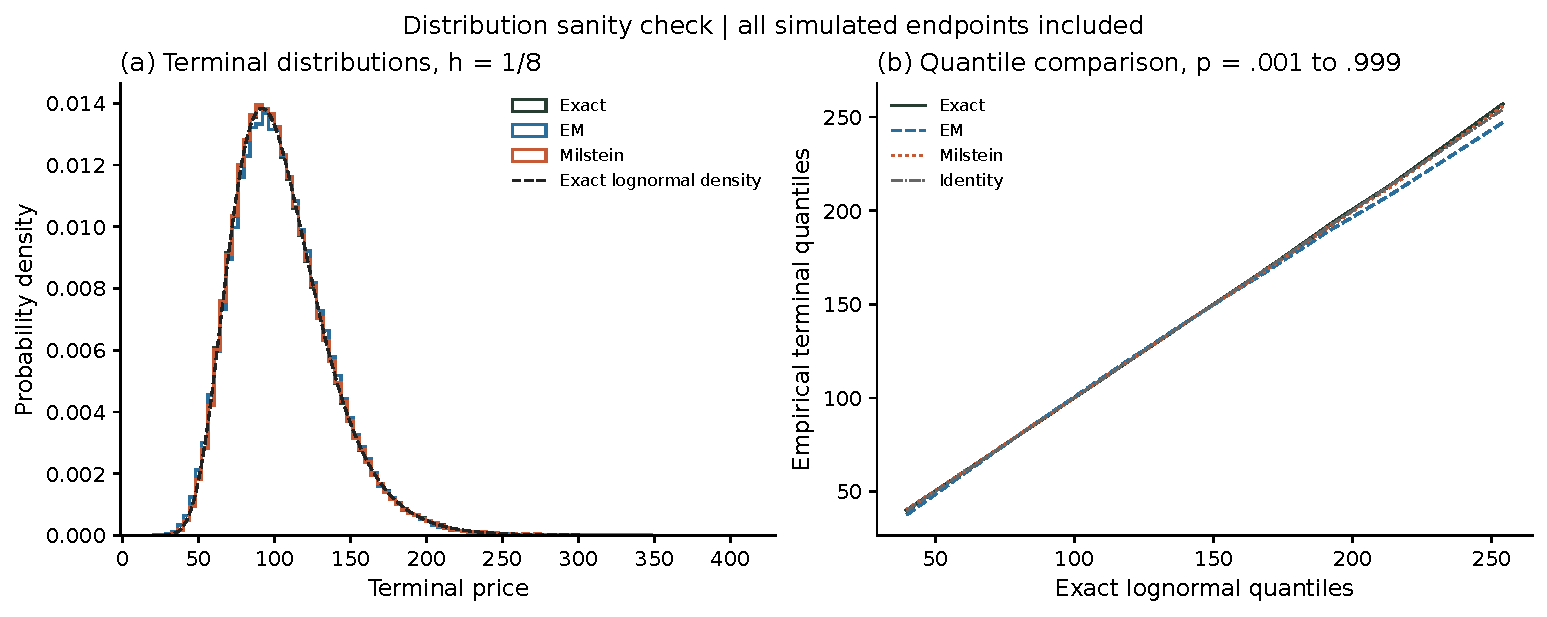
\includegraphics[width=.92\textwidth]{figures/gbm_distribution.pdf}
\caption{GBM 终值分布与精确对数正态定律的比较。直方图用于检查抽样形状，分位数提供更精细的分布比较。}
\end{figure}
\begin{table}[H]\centering\small
\caption{终值分位数；数值列使用 $h=1/8$。}\label{tab:gbm-quantile-cn}
\begin{tabular}{rrrrr}\toprule
$p$ & 对数正态理论值 & 精确模拟 & EM & Milstein\\\midrule
0.01 & 50.012 & 49.928 & 48.387 & 50.213\\
0.05 & 61.357 & 61.378 & 60.512 & 61.615\\
0.25 & 82.091 & 82.151 & 82.303 & 82.263\\
0.50 & 100.501 & 100.557 & 101.088 & 100.582\\
0.75 & 123.041 & 123.164 & 123.653 & 123.057\\
0.95 & 164.618 & 164.485 & 163.370 & 164.043\\
0.99 & 201.961 & 202.402 & 198.376 & 201.539\\
\bottomrule\end{tabular}
\end{table}

精确模拟的均值为 \GBMExactMean{}，方差为 \GBMExactVariance{}，均值区间为 \GBMExactMeanCI{}。理论均值为 105.1271，方差为 1040.7868。即使是精确模拟，经验矩和分位数仍会有抽样波动，不能把它们描述为离散误差。

当 $S_n>0$ 时，EM 一步更新得到负值的概率为
\begin{equation}
\mathbb P(S_{n+1}^{E}<0\mid S_n>0)
=\Phi\!\left(-\frac{1+\mu h}{\sigma\sqrt h}\right).
\end{equation}
对于 Milstein，配方得到乘子
\begin{equation}
\tfrac12\sigma^2(\Delta W+1/\sigma)^2+
\tfrac12+(\mu-\tfrac12\sigma^2)h.
\end{equation}
它只有在 $(\sigma^2-2\mu)h>1$ 时才可能为负。当前参数满足 $\sigma^2-2\mu=-0.01$，所以 Milstein 对任意 $h>0$ 都为正；一般参数下则不一定。

\begin{table}[H]\centering\small
\caption{GBM 负终值频率：每种方法、每个网格均模拟 160,000 条路径。}\label{tab:negative-frequency}
\begin{tabular}{ccc}\toprule
$N$ & EM：$S_N<0$ & Milstein：$S_N<0$\\\midrule
8, 16, 32, 64 & 0/160,000（0\%） & 0/160,000（0\%）\\
128, 256, 512, 1024 & 0/160,000（0\%） & 0/160,000（0\%）\\\bottomrule
\end{tabular}
\end{table}
保存的计数实际统计的是 $S_N\le0$，全部为零，因此严格负值的频率也为零。这是\emph{终值}频率，不是“路径中途曾经为负”的频率；本诊断没有保存 GBM 的所有中间价格。观察到零次负值不能证明 EM 保持正值。负价格可能影响非线性收益估计；将负值截成零也会改变算法。本文没有进行截断。

\newpage
\section{非仿真模型的数值结果}
\subsection{相对于数值参考的强差}
\begin{figure}[H]\centering
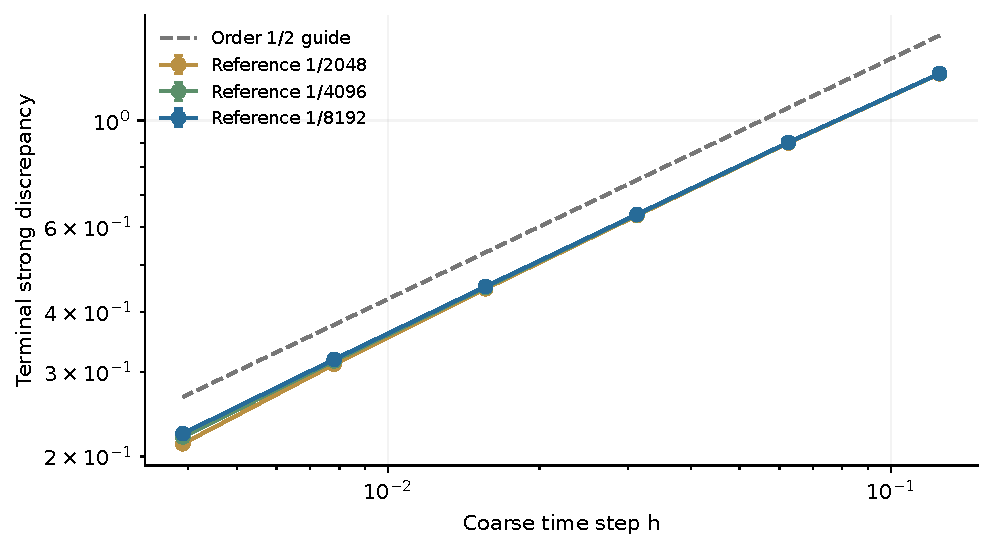
\includegraphics[width=.92\textwidth]{figures/report_nonaffine_strong.pdf}
\caption{相对于三层耦合 EM 参考网格的终值强差。参考是数值解，因此曲线不是相对于精确解的误差。}
\end{figure}
\begin{table}[H]\centering\small
\caption{相对于 $h_{\rm ref}=1/8192$ 的强差；给出 95\% 区间半宽。}\label{tab:na-strong-cn}
\begin{tabular}{rrr}\toprule
$h$ & $\mathbb E|S_h-S_{\rm ref}|$ & 最近一次参考差/强差\\\midrule
1/8 & $1.25354\pm0.00702$ & 3.2\%\\
1/16 & $0.90087\pm0.00489$ & 4.5\%\\
1/32 & $0.63818\pm0.00341$ & 6.3\%\\
1/64 & $0.45176\pm0.00241$ & 8.9\%\\
1/128 & $0.31854\pm0.00170$ & 12.6\%\\
1/256 & $0.22323\pm0.00119$ & 18.0\%\\
\bottomrule\end{tabular}
\end{table}

相对于最细参考，在 $\NAFitWindow{}$ 上的经验斜率为 \NARate{}。它与该窗口内大约半阶的强收敛行为一致。当粗网格接近参考网格时，曲线会弯曲：两个相近的离散解可能彼此很接近，但仍共同偏离连续时间 SDE 的解。

若 $S^\star$ 表示未知的精确终值，则反三角不等式给出
\begin{equation}
\left|\mathbb E|S_h-S^\star|-\mathbb E|S_h-S_r|\right|
\leq \mathbb E|S_r-S^\star|.
\end{equation}
右端未知。把 $r$ 换成更细网格，测到的是参考敏感性，而不是未知的精确误差。因此下文单独报告参考网格的变化，不把包含最细粗网格的斜率称为精确验证。

\newpage
\subsection{弱收益差}
\begin{figure}[H]\centering
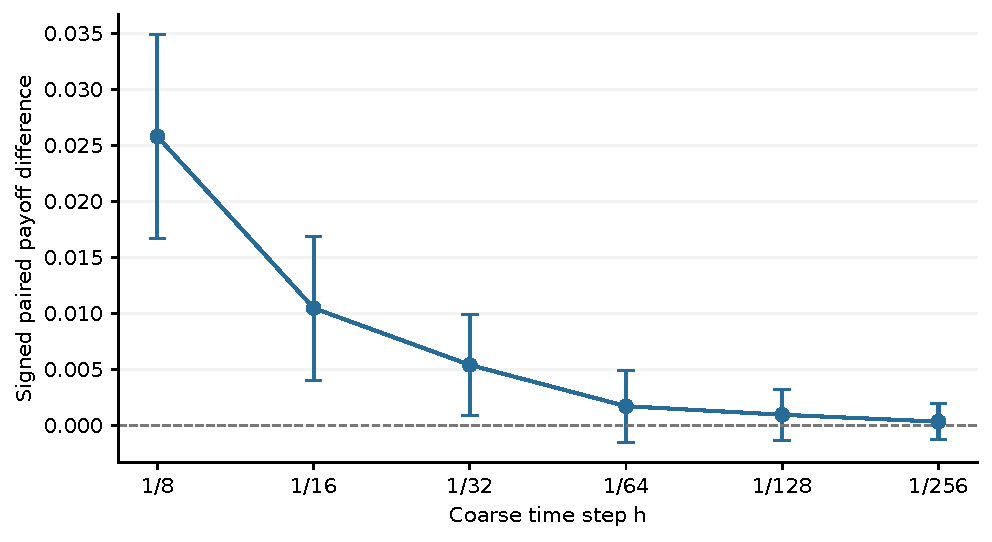
\includegraphics[width=.92\textwidth]{figures/report_nonaffine_weak.pdf}
\caption{相对于最细 EM 参考的看涨收益带符号配对差。误差棒为 95\% 抽样区间；零线帮助判断偏差符号是否可分辨。}
\end{figure}
\begin{table}[H]\centering\small
\caption{相对于 $h_{\rm ref}=1/8192$ 的带符号配对收益差。}\label{tab:na-weak-cn}
\begin{tabular}{rrrr}\toprule
$h$ & 估计偏差 & 95\% 区间 & 是否排除零\\\midrule
1/8 & 0.02579 & [0.01672, 0.03486] & 是\\
1/16 & 0.01048 & [0.00405, 0.01691] & 是\\
1/32 & 0.00540 & [0.00089, 0.00991] & 是\\
1/64 & 0.00172 & [-0.00148, 0.00492] & 否\\
1/128 & 0.00096 & [-0.00130, 0.00322] & 否\\
1/256 & 0.00034 & [-0.00124, 0.00192] & 否\\
\bottomrule\end{tabular}
\end{table}

\NAWeakInterpretation{}
收益函数在行权价处有一个折角，因此不能不加说明地套用光滑测试函数的弱阶理论。配对区间用于判断估计差异能否从抽样噪声中分辨；它们不包括数值参考的偏差。

\subsection{为什么 call payoff 比均值更有信息？}
连续模型满足 $\mathbb E[S_T]=100e^{0.05}$。但是，对数 EM 在每一个步长下也保留这个均值。令 $g_n=g(Y_n)$，在一步开始时 $S_n$ 和 $g_n$ 已知，而下一增量服从 $N(0,h)$，所以
\begin{equation}\label{eq:mean-preservation}
\begin{aligned}
\mathbb E[S_{n+1}\mid\mathcal F_{t_n}]
&=S_n e^{(\mu-g_n^2/2)h}\mathbb E[e^{g_n\Delta W_n^{(1)}}\mid\mathcal F_{t_n}]\\
&=S_n e^{(\mu-g_n^2/2)h}e^{g_n^2h/2}=S_ne^{\mu h}.
\end{aligned}
\end{equation}
重复这个条件期望计算便得到 $\mathbb E[S_N]=100e^{0.05}$。因此均值是有用的实现检查，但它对该方案没有时间离散偏差，无法显示弱收敛阶。

均值相同不代表期望收益相同。例如，价格总是 100，和以相同概率取 80 或 120 的价格，都有均值 100；但执行价为 100 的收益 $(S-100)^+$ 的期望分别为 0 和 10。Call payoff 能观察均值看不到的终值分布差异。它的期望没有被 log-EM 自动保持，因此改变步长可能产生真正的弱偏差。这就是它在本实验中作为非平凡弱观测量的原因；它不是唯一选择，也不保证每个网格都能测出显著偏差。

\newpage
\section{参考网格加密与验证}
\begin{table}[H]\centering\small
\caption{数值参考的耦合加密。}\label{tab:na-reference-cn}
\begin{tabular}{rrr}\toprule
参考加密 $N_a\to N_b$ & 强差 & 带符号收益差及 95\% 区间\\\midrule
2048 $\to$ 4096 & $0.05679\pm0.00030$ & -0.000023 [-0.000423, 0.000377]\\
4096 $\to$ 8192 & $0.04016\pm0.00021$ & 0.000094 [-0.000188, 0.000376]\\
\bottomrule\end{tabular}
\end{table}

\NAReferenceInterpretation{}
\begin{table}[H]\centering
\caption{最细非仿射网格上的布朗增量与状态诊断。}
\begin{tabular}{lrr}\toprule 项目 & 观测值 & 目标或范围\\\midrule
增量方差 1 & $1.221\times10^{-4}$ & $1.221\times10^{-4}$\\
增量方差 2 & $1.221\times10^{-4}$ & $1.221\times10^{-4}$\\
增量相关系数 & -0.699675 & $-0.700000$\\
抽样增量数 & 4,194,304 & 预先指定的第一批\\
总路径更新次数 & 1,484,000,000 & 所有网格\\
中间状态有限 & 通过 & $X$ 和 $Y$\\
价格为正且有限 & 通过 & 所有观测状态\\
\bottomrule\end{tabular}

\end{table}
两个布朗增量的方差目标都是 $h$，目标相关系数为 $-0.7$。这些诊断来自生成的细增量，而不是从生成器公式推断出来。状态检查包括中间更新，因为只有终值有限并不能排除中间步骤出现无效更新。

最细网格的均值为 \NAExactMean{}，95\% 区间为 \NAExactMeanCI{}；对应的未贴现收益估计为 \NAPayoff{}，区间为 \NAPayoffCI{}。后一个区间只描述最细离散模型的抽样不确定性；要评估其时间偏差，仍然需要参考加密表。

按照题目要求，本模型使用 EM。两维噪声下的 Milstein 方法还需要额外的交叉噪声项，不能直接把 GBM 的标量公式复制过来；本次比较不需要实现这个扩展。

\newpage
\section{讨论与结论}
GBM 实验支持三个结论。第一，与精确解进行共同路径比较，可以观察到 Milstein 的强收敛优势。第二，强阶和弱阶回答不同问题：尽管逐路径误差不同，两种方法对终值均值却有相同的一阶偏差。第三，分布和正值性检查提供了单个均值无法提供的信息。当 GBM 的精确转移可用时，对数价格模拟更直接；在价格上离散仍然是一个有用的受控验证实验。

对于非仿射模型，有界正波动率和指数价格表示使测试路径上的价格保持有限且为正。嵌套网格比较提供了加密收敛的证据，也揭示了数值参考会如何影响测得的阶数；它们不能给出精确误差。特别是，当收益区间包含零时，不能宣称已经测出弱收敛阶；当参考差异与粗网格差异相当时，对比较精度也必须保持谨慎。

主要计算取舍是路径数和时间分辨率之间的平衡。将 $h$ 减半，大约使每条路径的更新次数加倍；将 $M$ 增加四倍，蒙特卡洛标准误通常约减半。配对差和控制变量处理抽样部分，参考加密处理离散部分。增加路径数不能修复分辨率不足的参考，减小步长也不能单独消除抽样不确定性。

本文完成了题目第四方向的主要要求：精确解--EM--Milstein 比较、使用共同路径的强弱收敛、对数正态分布验证、抽样区间以及非仿射模型的嵌套参考检查。没有用确定性稳定性图或标量 Milstein 扩展替代这些要求。正值性诊断报告的是终值频率，并未统计所有中间更新；结论限于本文的参数、时间区间、误差范数、样本数和拟合窗口。

\subsection*{可复现性}
随附 Python 文件和保存结果记录了随机种子、样本数量和更新公式。本文使用已有实验结果，没有把它描述为一次新的完整模拟运行。附录给出核心更新和复现命令。

\subsection*{AI 致谢}
本报告使用 OpenAI Codex 辅助解释数学方法、开发和检查 Python 代码、完成数值计算，以及起草和修改报告。AI 也帮助改善了讨论和结果呈现的清晰度。

\begin{thebibliography}{9}
\bibitem{pack} \emph{Problem Pack: Five Suggested Directions for the ODE IVP Project}，课程作业文件，Direction~4，第 6--7 页。
\bibitem{higham} D.~J. Higham. An algorithmic introduction to numerical simulation of stochastic differential equations. \emph{SIAM Review}, 43(3):525--546, 2001.
\href{https://doi.org/10.1137/S0036144500378302}{doi:10.1137/S0036144500378302}。
\bibitem{kloeden} P.~E. Kloeden and E.~Platen. \emph{Numerical Solution of Stochastic Differential Equations}. Springer, 1992.
\href{https://doi.org/10.1007/978-3-662-12616-5}{doi:10.1007/978-3-662-12616-5}。
\end{thebibliography}

\newpage
\appendix
\section{Python 实现与复现}
下面的代码列出核心数学操作。可执行模块还实现了分批计算、控制变量预实验拟合、不确定性估计、诊断、导出和绘图；完整源码随报告提供。
\begin{lstlisting}[caption={核心 SDE 更新和共同路径误差统计。}]
import numpy as np

def coarsen(dw_fine, n_coarse):
    m, n_fine = dw_fine.shape
    assert n_fine % n_coarse == 0
    return dw_fine.reshape(m, n_coarse, -1).sum(axis=2)

def gbm_terminal(dw, s0=100., mu=.05, sigma=.3, T=1.):
    h = T / dw.shape[1]
    exact = s0 * np.exp((mu-.5*sigma**2)*T
                         + sigma*dw.sum(axis=1))
    em = s0 * np.prod(1 + mu*h + sigma*dw, axis=1)
    mil = s0 * np.prod(1 + mu*h + sigma*dw
              + .5*sigma**2*(dw*dw-h), axis=1)
    return exact, em, mil

def log_em_step(x, y, dw1, dw2, h):
    # 两个右端都使用旧时刻的数值。
    sigmoid = np.exp(-np.logaddexp(0., -y))
    g = .1 + .4*sigmoid
    x_new = x + (.05-.5*g*g)*h + g*dw1
    y_new = y + 2*(-.2-y)*h + .6*np.hypot(1.,y)*dw2
    return x_new, y_new

def mean_ci(values):
    m = len(values)
    mean = np.mean(values)
    half_width = 1.96*np.std(values, ddof=1)/np.sqrt(m)
    return mean, mean-half_width, mean+half_width

# 从独立标准正态数生成相关布朗增量：
# dw1 = sqrt(h)*z1
# dw2 = sqrt(h)*(rho*z1 + sqrt(1-rho**2)*z2)
# 强误差：mean_ci(abs(s_coarse-s_reference))
# 弱误差：mean_ci(maximum(s_coarse-100,0)
#                -maximum(s_reference-100,0))
\end{lstlisting}
\noindent 在原项目目录中运行：
\begin{lstlisting}[numbers=none]
python -m pip install -r requirements.txt
python run_all.py

# 在不重新模拟的情况下核对已有结果：
python verify.py
\end{lstlisting}
\noindent 在本目录中编译中文报告：
\begin{lstlisting}[numbers=none]
tectonic Coursework_Undergraduate_中文.tex
\end{lstlisting}
\noindent\small 原项目的 \texttt{results/} 保存机器可读的表格和日志，\texttt{figures/} 保存矢量 PDF 和 PNG 图。附录代码用于解释核心算法；完整复现需要两个模拟模块，而只重建报告表格不会重新模拟路径。
\end{document}
